\section{Ταξινόμηση άρθρων}
\label{sec:classification}
Για την ταξινόμηση των εισερχόμενων άρθρων στο σύστημα μελετήθηκαν δύο υλοποιήσεις. Η πρώτη αφορά την κατασκευή ενός \emph{Multi-Layer Perceptron} και η δεύτερη αφορά το \emph{finetuning} του ελληνικού BERT \cite{greek-bert} μοντέλου.

\subsection{\emph{Multi-Layer Perceptron}}
Για την κατασκευή του \emph{MLP} χρησιμοποιήθηκε η βιβλιοθήκη \emph{Keras} \cite{keras}. Τα βήματα που ακολουθήθηκαν για την κατασκευή του μοντέλου μπορούν να βρεθούν αναλυτικά στην \emph{developer} σελίδα της \emph{google}\footnote{\url{https://www.google.com/}} για \emph{ταξινόμηση κειμένου}\footnote{\url{https://developers.google.com/machine-learning/guides/text-classification}}. Πιο συγκεκριμένα, για το μοντέλο επιλέχθηκε αρχιτεκτονική δύο κρυφών επιπέδων, \autoref{fig:mlp-arch}, και για στην έξοδο εφαρμόζεται συνάρτηση \emph{softmax} για την κανονικοποίηση των πιθανοτήτων και το άθροισμα τους στη μονάδα.

Το μοντέλο εκπαιδεύτηκε σε μία σειρά από άρθρα, τα οποία αποκτήθηκαν με τη μέθοδο που παρουσιάστηκε στο \autoref{sec:soup}. Αρχικά, εφαρμόζεται \emph{tokenization}, η διαδικασία  χωρισμού των παραγράφων σε λέξεις ή ακολουθίες λέξεων (σύμβολα, το λεξιλόγιο του μοντέλου), για καλύτερη γενίκευση της σχέσης μεταξύ των λέξεων και των ετικετών και στη συνέχεια μετατρέπονται σε διανύσματα (\emph{vectorization}). Για το \emph{vectorization} χρησιμοποιείται ο αλγόριθμος \emph{TF-IDF}. Με τη διαδικασία αυτή παράγεται το λεξιλόγιο του μοντέλου. Στο τέλος ενδέχεται να έχουν παραχθεί χιλιάδες σύμβολα/λέξεις στο λεξιλόγιο. Από αυτά τα χιλιάδες σύμβολα δεν συνεισφέρουν όλα εξίσου στην κατηγοριοποίηση της εισόδου. Επομένως, μπορούν να παραλειφθούν εκείνα τα οποία έχουν πολύ μικρή σημασία για τη πρόβλεψη του μοντέλου. Η συνάρτηση που χρησιμοποιήθηκε για την εξαγωγή της σημαντικότητας των συμβόλων είναι η \emph{f\_classif}\footnote{\url{https://scikit-learn.org/stable/modules/generated/sklearn.feature_selection.f_classif.html}} και επιλέχθηκαν τα πρώτα $20.000$. 

\begin{figure}[!ht]
  \centering
  \captionsetup{justification=centering}
  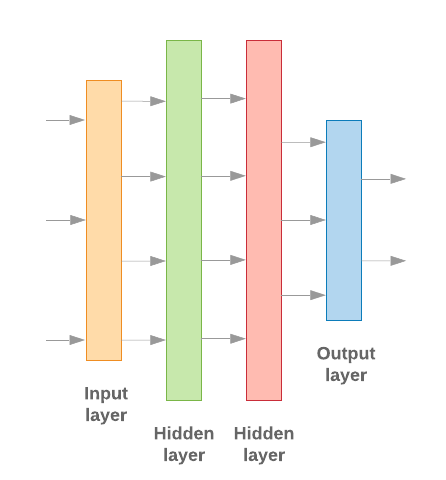
\includegraphics[width=10cm]{images/chapter4/mlp-arch.png}
  \captionsource{Αρχιτεκτονική μοντέλου \emph{MLP}}{\url{https://developers.google.com/machine-learning/guides/text-classification/images/LinearStackOfLayers.png}}
  \label{fig:mlp-arch}
\end{figure}
\noindent

\subsection{\emph{Greek-Bert}}
Για την περαιτέρω εκπαίδευση του ελληνικού μοντέλου \emph{BERT}\footnote{\url{https://huggingface.co/nlpaueb/bert-base-greek-uncased-v1}} χρησιμοποιήθηκε η βιβλιοθήκη \emph{Torch} \cite{torch} σε συνδυασμό με την βιβλιοθήκη \emph{Transformers} \cite{transformers}. Το ελληνικό \emph{BERT} μοντέλο αποτελείται από $12$ \emph{attention heads}, $12$ \emph{hidden layers} και αποτελείται από λεξιλόγιο $35000$ λέξεων. Σε αυτή την υλοποίηση το μοντέλο εκπαιδεύεται με την ίδια σειρά άρθρων, όπως και το \emph{MLP}. Για την μετατροπή των παραγράφων σε \emph{tokens} χρησιμοποιήθηκε ο προκαθορισμένος \emph{tokenizer} του αρχικού μοντέλου.